\chapter{System Architecture}
\label{chap:System Architecture}

% 6 pages
The main goal of this work is to apply ML-based interpolation techniques to the topic of UHI detection to improve data availibility and compare different interpolation techniques that are based on traditonal (statistical) and ML-based approaches. ML-based models first of all need a lot of data to be trained and validated with, and after deployment need access to relevent real-time data, if near real-time capabilities are desired. In the context of smart city, such ML-based interpolation models could be used to improve data availibility by interpolating missing/unavailable data such as LST readings under cloudy conditions, and be incoperated into a service that other services, like a UHI detection service, could further rely on, without the need to implement interpolation techniques themselves. This could reduce costs to develop such depending services, as they no longer need to deal with missing data themselves while also improving interpolation results with well-trained and designed models. First, we need to take a look at how such a service fits into existing smart city architectures.

\begin{figure}[h]
    \centering
    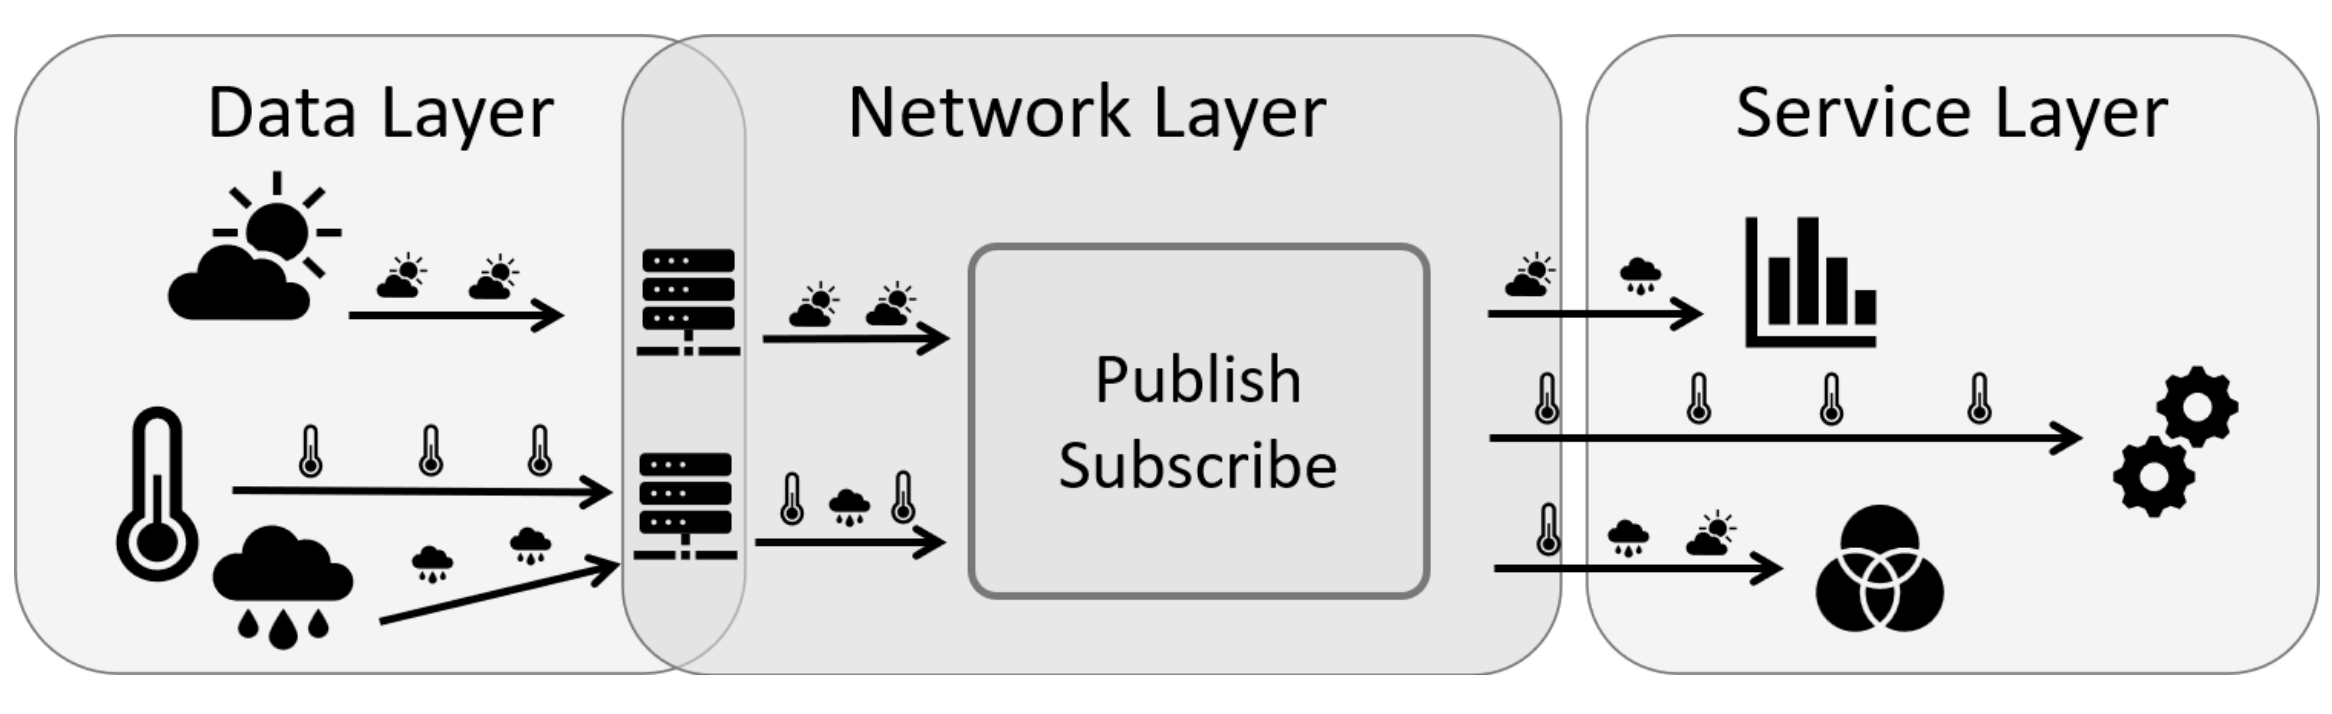
\includegraphics[width=\textwidth]{images/expose-system-architecture.png}
    \caption{In the data layer (left), a wide variety of environmental data is collected with the help of multiple sensors. These are connected to their citizen-owned local base stations, which manage access rights and forward collected data to subscribed services (right) via the decentralized publish-subscribe in the network layer (center).}
    \label{fig:system-architecture-overview} %todo: create graphic of the 4 layers instead
\end{figure}

\section{Architecture Layers of Smart Cities}

 The most generalised architecture of a smart city consists of four layer, the sensing layer, transmission layer, data management, and application layer~\cite{silva2018towards}. In this work, we focus on the sensing layer, dealing with topics such as correct sensor placement and underlying sensor footprints, and the application layer, which accesses available data via data management services to provide additional services to the city and its citizens. For the data transmission and data management layers, there already exist different technologies and service offerings, that aim at solving the underlying problems, e.g. network bandwidth, network availability, sensor discoverability, handling the massive amounts of data that is already or will be collected in the future, and many more. For the communication and discovery of sensor nodes, one solution could be SkipNet~\cite{harvey2002skipnet}, an overlay network focused on discoverability while also protecting privacy, with which the data transportation layer could be desinged as a peer-to-peer (P2P) network. Other research focuses on the data accessability and discoverability, by making data accessible for everyone, not only for economic partners in a closed-off system. Examples would be the Smart Networks For Urban Citizen Participation (SANE) initiative~\cite{bornholdt2019sane}, which... Figure \ref{fig:system-architecture-overview} shows the architecture of the SANE system.

% Todo: potentially write more about SANE and data marts etc.

\subsection{Sensing Layer}
\label{subsec: Sensing Layer}

% todo: take a closer look at sensing layer with challenges like sensor placement, uncertainty etc.

The goal for the sensing layer is to monitor the surrounding environment and capture key data for further analysis and decision making. It consists of many different types of physical and virtual sensors. The first group of sensors are the physical sensors, which are placed directly inside the environment. Wireless sensor networks (WSN)~\cite{dargie2010fundamentals} have seen a lot of attention for many different applications such as `military sensing, physical security, air traffic control, traffic surveillance, video surveillance, industrial and manufacturing automation, distributed robotics, environment monitoring, and building and structures monitoring'~\cite{chong2003sensor}. The challenges for WSNs primarily depend among other things on the deployment. An ad-hoc WSN has energy and bandwidth contraints due to the usage of batteries as power sources.
In contrast, sensors that are permanetly installed, either stationary or on a moving target, and connected to a constant power source don't have this constraints. This approach could be used for smart cities to reduce waste and guarantee representative measurements via correct sensor placement. In the case of stationary sensor networks though, the initial deployment and following maintenance cost can be substantial~\cite{chapman2015birmingham}.\\
In recent years, low-cost sensors (LCS) in combination with sensor networks have enabled fine-granular real-time monitoring of urban environments~\cite{grimmond2006progress, rundel2009environmental}, although the quality of individual low-cost sensors can be questionable~\cite{castell2017can}. In general, LCSs can improve data availibility and support analysis, but do not substitute well-calibrated reference instrumentation~\cite{lewis2018low}.
% could also discuss low cost sensors

\subsubsection{Stationary Sensor Types}
There are many different types of environmental features that can be measured directly inside an urban area. The types of measurements that can be observed are among others: air temperature, humidity, atmospheric pressure, reactive gaseous air pollutant (CO, NOx, O$_3$, SO$_2$), particulate matter (PM), greenhouse gases (CO$_2$, CH$_4$), percipitation, solar radiation, wind speed and direction, anthropogenic heat, noise, sky-view factor, heat fluxes and many more. % Todo: Soil
Correlations between these features can vary greatly based on surrounding factors. In order to better understand these correlations, many empirical studies have studied the influence of meteological factors on features such as PM~\cite{tai2010correlations}. Additionally, many fields of statistics have specialised on topics such as statistics in climatology~\cite{von2002statistical}, geostatistics~\cite{trangmar1986application} and more.\\
All sensor readings that are taken by physical sensors are singular data points. Additionally to the type of measurement taken and the actual value observed, physical sensor readings include the physical location of the sensor, e.g. latitude, longitude and altitude, the type of sensor used to take the measurement, and the sampling rate. For air temperature, the sampling rate could be an average temperature measured over five minutes, whereas percipitation might be measured by collecting rain for certain periods of time and then measuring the amount of rain collected. The sensor type is important, as different types of sensors can produce different qualities of measurements, e.g. LCS compared to callibrated reference-grade high cost sensors, and perform better or worse based on the meteological conditions, e.g. worse performance at low temperatures, high humidity etc. Due to the placement directly inside the environment, (near) real-time observation and high temporal resolution are generelly possible, but might be influenced by factors such as network availability. The spatial resolution highly depends on the number of sensors deployed and the correct placement of the sensors. The correct placement has a direct influence on the footprint of the sensor~\cite{leclerc2014footprints} and the representativness of the measurement taken for the underlying and surrounding area~\cite{oke2006guideline}.\\
One downside of the placement directly in the environment the sensors are observing, is the exposure to environmental influences such as heat, humidity, or pollution, that can decrease the lifetime of a sensor and may require more frequent maintenance or replacement.

% Todo: list of sensors with downsides

- discussion premium vs low-cost sensors
- discussion static data incorporation -> NDVI from geoportal via data management layer

- P2,5: highly depends on air flows
- humidity: needs to be replaced more often due to pollution
- temperature

\subsubsection{Mobile Sensor Types}

% describe how mobile sensors can be used to complement stationary sensors
- mobile Windmessungen mit einem SODAR - einem akustischen Windmesssystem -, Vergleichsmessungen an einer stationären Messstelle auf
- Profilmessfahrten

\subsubsection{Remote Sensing}
% remote sensing

In comparison to stationary sensors that are installed directly in the environment they are observing, remote sensing describes the process of observing a target environment from afar~\cite{campbell2011introduction}. In climatology, remote sensing is used to collect meteological data via satellites, planes or ballons by either capturing image data, that can be used to identify things like cloud and land coverage, by measuring passive radiation, or by actively sending out microwaves or using LIDAR to detect features such as surface temperature, e.g. LST data. Remote sensing comes with its own set of advantages and challenges.\\
The major upside of sensors moving way above ground is the high spatial coverage, that allows for meso- and planetary-scale anaylsis of weather phenomena. Another upside is the great data availibility, as many satellite providers, such as ESA..., publish their satellite data. This creates many research opportunities, and many services directly rely on these measurements (todo list).\\ % gridded data
% remote sensing challenges
Remote sensing also comes with some downsides. The primary downside is the low spatio-temporal resolutions. Weather satellites usually are not orbit-stationary and move around earth on a predetermined orbit. As a consequence, satellites only pass over each individual area a couple times a day, making real-time applications for currently unobserved areas impossible. Additinally, the spatial resolution can be too low for micro-/local-scale analysis, with typical LST resolution spanning from 1 km$^{2}$ to tens or even hundreds of km$^{2}$ per data point/grid field. In the atmosphere, there is also a lot of environmental noise, like radiation, that can have a negative influence on the measurement accuracy. Another disturbing factor can be clouds or other types of particles like rain, that absorb radiation/microwaves sent from the sensors, traditionally making measuring under cloudy/rainy conditions either impossible (example) or less accurate (example), by instead relying on outgoing radiation from the surface. These restrictions highly depend on the sensor used, as different sensors use different 
sensors use different technologies, e.g. microwaves with different wave lengths or higher resolution sensors.

% todo: potentially more to the downsides of each sensor type / overview of types of satellites

\subsubsection{Modelling of the Sensing Layer}

A model is an abstraction of the real world that helps us analyse and understand complex problems. In the context of UHI detection, we can use model climate on a bigger scale, or the micro-slimate inside a city, to better understand and capture influences. In this work, we focus on ...\\
% Todo
One major consideration in this context, what type of data is used to validate and train the ML models. The options in this case are either climate models which simulate data, or capturing/collecting real-world data. Due to the complexity and limitations of simulation, this work only focuses on collecting real-world data.
% Todo


% The \textit{sensing layer} consists of many different data sources. In the context of temperature sensing and prediction, this could include single (inexpensive) sensors such as the popular BMP280 \footnote{https://www.bosch-sensortec.com/products/environmental-sensors/pressure-sensors/bmp280/}, private weather stations such as sold by Netatmo \footnote{https://www.netatmo.com/en-gb/weather/weatherstation} hidden behind an API \footnote{https://dev.netatmo.com/apidocumentation/general}, public weather station data such as from the Deutscher Wetterdienst (DWD) \footnote{https://www.dwd.de/} which offer an API and historic weather data, or other geologically relevant data such as zoning plans which, in the case of the city of Hamburg in Germany, can be accessed via an OpenData platform provided by the State Office for Geoinformation and Surveying Hamburg \footnote{https://geoportal-hamburg.de/geo-online/}. In order to gain detailed insights into urban microclimates, we need fine-grained spatial and temporal data. As managing and maintaining such a large sensor network as a single entity can be quite challenging and cost intensive \cite{chapman2015birmingham}, we rely primarily on crowdsourced sensor data, in this case climate-related, from citizens, that give access to their personal sensors that they f.e. installed at home. This approach has been shown to work well in the densely populated urban area of Berlin, Germany \cite{meier2017crowdsourcing}, with the main challenge being data quality assessment due to faulty data from either broken, wrongly configured or wrongly installed sensors. The different data sources provide data streams which are then ingested by our interpolation service. Main challenges are the uncertainty in networks, such as single sensors or APIs not being available due to network interruptions, and the integration of many heterogeneous data sources that can contain data in different formats, time intervals or units of measurement etc.\\
% The \textit{network layer} is responsible for integrating these different data sources in a consistent and reliable way and making them available for other services. The different sensors present in the data layer might have different vendors and programming interfaces, be located behind (vendor specific) APIs or are unreliably accessible due to unstable networks in edge environments. The network layer can be designed as a peer-to-peer (P2P) network based on the SkipNet approach \cite{harvey2002skipnet}, that utilizes the lookup efficiency of distributed hash tables and adds support for value-based range queries based on prefixes and attribute-value pairs. Another challenge in the context of the network layer, especially in the context of this paper, is also the integration of mobile sensors, which might not be constantly connected to a network while moving.\\

\subsection{Data Transportation Layer}
Todo (small)

\subsection{Data Management Layer}

% Todo: write
How to handle such large amounts of data
Connection to other APIs
Dealing with the heterogenity of data
modeling uncertainty of data

\subsubsection{Integrating Static Data}
\label{subsubsec: integrating static data}

Next to sensor readings captured for a given area, there are also other types of information that could be useful for ML applications. Alonso and Renard~\cite{alonso2020new} used these additional indexes to predict air temperature:

% Todo: make into table on one page
\begin{itemize}
    \item Vegetation Index
    \begin{itemize}
        \item Normalized Difference Vegetation Index (NDVI)
        \item Soil Adjusted Vegetation Index (SAVI)
        \item Enhanced Vegetation Index (EVI)
        \item Tasseled Cap Transformation greenness (GVI)
        \item Density of low vegetation
        \item Density of medium vegetation
        \item Density of high vegetation
    \end{itemize}
    \item Water Presence Index
    \begin{itemize}
        \item Modified Normalized Difference Water Index (MNDWI)
        \item Normalized Difference Water Index (NDWI)
    \end{itemize}
    \item Moisture Index
    \begin{itemize}
        \item Tasseled cap Transformation Wetness
        \item Normalized Difference Moisture Index (NDMI)
    \end{itemize}
    \item Bare Soil Index
    \begin{itemize}
        \item Normalized Difference Bareness Index (NDBaI)
        \item Bare Soil Index (BI)
        \item Enahnced Build-Up and Bareness Index (EBBI)
        \item Density of bare soil
    \end{itemize}
    \item Radiation Index
    \begin{itemize}
        \item Spectral radiance
        \item Emissivity
        \item Tasseled Cap Transformation Brightness
    \end{itemize}
    \item Building Index
    \begin{itemize}
        \item Normalized Difference Build-Up Index (NDBI)
        \item Urban Index (UI)
        \item Index-based Build-Up Index (IBI)
        \item Building Density
    \end{itemize}
    \item Topographic
    \begin{itemize}
        \item Slope (°)
        \item Exposure
        \item Curvature
    \end{itemize}
    \item Urban morphology
    \begin{itemize}
        \item Sky View Factor
        \item Standard Deviation (STD) of Building Height (building height variation)
    \end{itemize}
    \item Land use
    \begin{itemize}
        \item Distance to railway tracks
        \item Distance to points of tourist interest
        \item Distance to subway entrances
        \item Distances to fountains
        \item Water area
    \end{itemize}
\end{itemize}

These types of data can be sourced either directly via satellites like LiDAR or Landsat 8, or via geoportals that publish such data, like the State Office for Geoinformation and Surveying Hamburg~\footnote{\url{https://geoportal-hamburg.de/geo-online/}} on a regional basis or the EU Inspire Geoportal~\footnote{\url{https://inspire-geoportal.ec.europa.eu/}} on a continental basis.

\subsubsection{Integrating External APIs}

Currently, there exist some cities that already operate open-source sensor networks that usually act as a middleware to upload and retrieve sensor data and offer additonal functionalities like alert or notifications. A detailed list of case studies is provided in \ref{sec: smart city case studies}. Next to city specific initiatives, there exist also independent sensor network platforms or initiatives. These are either operated by vendors of f.e. IOT devices, or by open-source communities. In the following, one vendor and one open-source community project is portraied in more detail:\\
\\
\textbf{Netatmo}: Netatmo~\footnote{\url{https://www.netatmo.com/}} is a French Smart Home Company that was founded in 2011. It has a large smart home assortment including cameras, door bells, smoke detectors, thermostats and weather stations among others. In the context of collecting meteological data, the smart weather products are of particular interest. These include a smart weather station that collects air temperature, humidity and air pressure, an anemometer that collects wind speed and direction, and a rain gauge. The sensor specifications, as reported by the vendor himself, is reported in Table \ref{tab: netatmo sensor specs}.\\
Complementary to its smart products, Netatmo also operates a weather platform and a developer portal. The weather platform offers a weather map~\footnote{\url{https://weathermap.netatmo.com/}} containing the measurements of connected weather stations accross the whole world for air temperature, precipitation, and wind speed and directon. The developer portal~\footnote{\url{https://dev.netatmo.com/apidocumentation}} offers a way to programmatically access all sensor measurements via a REST API. In this work, we later use this REST API to collect sensor data, as discussed in Chapter \ref{chap:preparations data sets}.

% precisions
% Please add the following required packages to your document preamble:
% \usepackage{booktabs}
\begin{table}[]
\begin{tabular}{@{}lllll@{}}
\toprule
Measurement    & Unit    & Measurement Range      & Precision  & Recording Frequency              \\ \midrule
Temperature    & °C      & -40°C to 65°C          & 0.3°C   & averaged over 5 min              \\
Humidity       & \% (RH) & 0 to 100\%             & 3\%     & -                                \\
Air Pressure   & mbar    & 260 to 1160 mbar       & 1mbar   & -                                \\
Noise          & dB      & 35 to 120 dB           & -       & -                                \\
Wind Speed     & m/s     & 0 to 45 m/s (160 km/h) & 0.5 m/s & every 6 sec, averaged over 5 min \\
Wind Direction & °       & 0 to 359°              & 5°      & every 6 sec, averaged over 5 min \\
Rainfall       & mm/h    & 0.2 to 150 mm/h        & 1mm/h   & every 5 min (bucket is emptied)  \\ \bottomrule
\end{tabular}
\caption{Netatmo Sensor Specifications (Vendor reported)}
\label{tab: netatmo sensor specs}
% todo: adjust to page size, maybe move to dataset chapter
\end{table}

Next to commercial vendors, there also exist OpenSource projects which operate and develop sensor platforms independently:\\
\\
\textbf{Sensor Community}: Sensor.Community~\footnote{\url{https://sensor.community}} is an open-source community driven project that aims to collect Open Environmental Data. The project is part of the initiative OK Lab Stuttgart~\footnote{\url{https://codefor.de/stuttgart/}}, which is run by a group of volunteers that ...
13.500 sensors world-wide, open source\\
% sensors used SS0 etc. precisions
- BME280
- SHS 
\\
% potentially more examples.
Most of the solutions have in common, that ...
- accounts, request quotas, historical data?

But, they also differ at...
- no common REST standard, no shared accounts, sensor descriptions (placement)

\subsection{Application Layer}

The application layer contains services which utilize data provided by the data management layer to provide services for the city and its citizens. As part of this layer, services could be build that aggregate data streams coming from the data management layer and use ML to improve the data quality by detecting outliers, reducing bias, interpolating missing data etc. The improved data could then be published and other services that would otherwiese rely on the raw data streams and potentially need to implement their own outlier detection or interpolation of missing data techniques, instead simply subscribe to the externally managed service. This could lower the barrier to entry for developers with less available resources, financially or domain-knowledge wise, and generelly allow developers/service providers to allocate their resources to other areas like user experience (UX) and usability compared to the maintenance of complex ML-based services.\\
In the context of this work, we focus on the topic of UHI detection. In this context, there could be a UHI detection service that ingests real-time data streams from the data management layer and notify citizens if an UHI is detected in or predicted for a particular urban area. As the main challenge for UHI detection lies, next to the definition of urban and rural reference areas, on the gathering of a comprehensive temperature map that allow UHI detection algorithms to work, in this work we primarily focus on creating and evaluating an air temperature map service, that enables the detection of CUHIs and could also be used as a foundation for other services in a smart city, like plant watering systems, smart healthcare and more.

\section{Applications for Machine-Learning}

The data management layer publishes historical data and real-time data streams for application service to ingest. Generally, ML can be used for the following tasks in different variations:

\begin{itemize}
    \item Classification
\end{itemize}

In this context, 

% todo
This section is about where ML could be used (Land cover, )

- comparison to NLP -> pipeline vs singular model (NLP pipeline vs ChatGPT)

applications:
- all-in one solution (all features included) -> huge DL model with billions of parameters (ChaptGPT)
    - not feasible in this thesis
- pipeline solution (use ML models incrementally and build upon results)
    - similar to NLP
    - feasible for specific topics
    - bottom-up approach (use ML to increase the amount of available data)

- types of ML utilisation
    - utlier detection
    - classification
    - regression
        - interpolation of missing data
        - prediction of future data

\subsection{Parallels to Natural Language Processing}

NLP pipeline (stemmer, lexer, etc.)
vs single model (ChatGPT) - neural network with billions of parameters

% continous improvements


\section{Smart City Case Studies}
\label{sec: smart city case studies}
% get from data management list...

Many european cities, like Amsterdam, Barcelona, London and Stockholm, have developed their own smart city strategies and platforms. In the following, we take a closer look at the steps each city has taken:\\
\\
\textbf{Barcelona, Spain}: Barcelona operates the `Sentilo' platform~\footnote{\url{http://www.sentilo.io/}}, an open-source smart city platform that aims to break down informatioal silos inside the city to provide unified access to the data available. It currently contains more than 27.000 sensors~\footnote{\url{http://connecta.bcn.cat/connecta-catalog-web/stats/} (\textit{Accessed: 23.03.2023})}. It offers a modular and extensible architecture, high performance and scalability, alerts, stats, triggers, a simple REST API to send and receive sensor data, and is cross-platform by being build with Java, Redis and MongoDB.\\
%Todo: move to section with case studies
\\
\textbf{Amsterdam, Netherlands}: Amsterdam utilizes sensors to run an extensive smart lighting system, that\\
\\
\textbf{London, England}: More infos\\
\\
\textbf{Stockholm, Sweden}: More infos\\
\\
More honorable mentions from outside the EU:\\
\\
\textbf{Singapore}: more infos\\
\\
\textbf{San Fransico, US}: more infos\\
